\documentclass[•]{article}
\usepackage{hyperref}
\usepackage{url}
\usepackage{listings}
\usepackage{graphicx}
\usepackage[normalem]{ulem}
\title{Optimise D4P}
\begin{document}
	\maketitle
	\begin{abstract}
	\sout{This is the abstract containing the main content of the dissertation document. Abstract is with title page.}
	\end{abstract}
	\pagebreak
	
	\sout{Declaration of understanding of the University's plagiarism guidelines.	}
	
	\pagebreak	
	
	\sout{The length of the document should be 40 -- 50 pages in total and no shorter than 20 pages.}
	\section{Introduction}
	\sout{What's scientific workflow. What's workflow execution systems. What's dispel4py and why dispel4py. Current weaknesses / points can be optimized. The optimizations taken, and they enable further optimization and / or new semantics / dynamics. \\
	What we are going to optimize, and high-level descriptions of them. \\
	How the following document will be organized.}
	
	We report the exploration of improvements to a workflow management system that enables scientific methods to be encoded using data streaming. We report and evaluate a prototyping dynamic mapping of processes onto computational platforms.
	
	The prevalence of workflow systems as a means of ongoing computational and data driven methods motivates this work. The nature of these systems and their data-streaming variants are introduced to set the context for the experiments. We then introduce dispel4py as well as possible enhancements to it, and briefly describe our design to tackle them.
	
	Science and researchers have gone through many eras and stages, and are facing a new paradigm today - data-intensive science \cite{hey2009fourth}. Many current research campaigns involve producing large quantities of data and analysing them. As always, researchers need to develop methods themselves and then perform computation and analyse the results. Consequently researchers need flexible tools to help organise, implement and perform their methods. Here is how workflows and workflow management systems join the story: researchers can describe their methods by means of workflows and execute them in a workflow management system.
	
	A scientific workflow (``workflow'' for short) is a technique used to organize and manage scientific computational jobs. By using scientific workflow, each computational job is decomposed into several (sub-)tasks which are connected by their dataflows (data dependencies). Hence, every workflow can be easily re-designed to suit specific needs by modifying its (sub-)tasks. Moreover, each (sub-)task can be seen as a module which can be developed independently, and they can be reused in different workflows so researchers can easily design new workflows by selecting and combining different modules.
	
	The software system / framework used to execute scientific workflows is called workflow management system (WMS). Researchers only need to provide the workflow and relevant input data, then the rest of the story will be automated by the WMS. Usually WMSs will parse the given workflow and map / assign tasks to some kinds of distributed computation platforms, such as clusters.
	
	Dispel4py is a data-streaming workflow management system written in Python \cite{doi:10.1177/1094342016649766}. It doesn't introduce new execution platforms, but maps the workflow into some existing platforms such as MPI \cite{MPI_forum} or Apache Storm \cite{apache_storm}. As Python is widely available, the computers / servers on which the execution will happen don't need extra configurations. That said, as long as the libraries that tasks / PEs used are installed, dispel4py can take control of the whole executing process and use the platform existing with no require of users' attention. If the tasks / PEs are written completely in Python, then no configuration is needed at all.
	
	Currently, as far as we know, the workflow going to execute should be constructed solidly before its execution and is not subjected to change during its execution in most WMSs (which is all of the data-streaming WMSs and most of the task-oriented WMSs [the differences between data-streaming WMSs and task-oriented WMSs will be detailed in the ``Background'' section] with only a few exceptions, such as DAGMan for Condor \cite{couvares2007workflow}) and the deployment (i.e. which node will execute which sub-task) happens at the beginning of the execution, which means the workflow as well as its deployment will be static during the execution. However, some computations can be represented more naturally in a dynamic way (for example, the sieve of Eratosthenes, which will be detailed in the ``Dynamic Expansion'' section) and some nodes (especially the ones near the end of the workflow) are actually waiting for a long time before data come. As a consequence, it may save time or resources not to deploy all nodes in the beginning and may save nodes (therefore lower computational resources needed) if we can collect and re-allocate nodes that have finished producing outputs. To tackle this weakness, we extended dispel4py to give it the ability to dynamically / incrementally deploy (sub-)tasks to computer nodes and a new semantics, \textit{dynamic expansion}, to workflows. In the meantime, our new system keeps backward compatibility so that existing workflows can still be correctly executed.
	
	The ability to deploy (sub-)tasks to computer nodes only when needed is called \emph{incremental deployment} by us. We introduce a coordinator node that knows the global structure of the workflow and is in charge of nodes deployment, and degrade the rest of the nodes to executors that only know themselves and their neighbours (i.e.\ the nodes its input and output connections are connected with). Every time an executor needs new output targets, it requests that node and gets response from the coordinator. After all executors have finished their work (i.e.\ no more inputs and outputs), they will all be shut down by the coordinator (and the coordinator also shuts itself down), so the whole execution is then finished. We use carefully designed signals / communications (which will be detailed in the ``Incremental Deployment'' section) to ensure the execution and shut-down process's correct execution.
	
	The new semantics to grow the workflow dynamically according to certain rules is called \emph{dynamic expansion}. In order to keep backward compatibility, we add a special mark (implemented as a \lstinline|property| with default value) to the Processing Element (PE) indicating whether or not the task can be further expanded. In order to encode the expansion rules, we add special connections (called \emph{circuit connection}) and corresponding methods to define them. The details will be described in the ``Dynamic Expansion'' section.
	
	Introducing these two new extensions enables us (or other researchers / developers) to make further optimisation and extensions. For example, in the original dispel4py system, we can only collect performance data of past runs and use them to direct the deployment of future runs; but now, we can also collect the performance data during the incremental deployment (i.e. on-the-fly) and use these data to aid the following deployment of the same execution.
	
	The remaining part of this document will be organised as follows: first, we will present some terminology which may lead to confusion if not stated clearly; following that, we will present necessary background information; then we will detail the extensions we have done in separate chapters; after that, we will present the measurement and evaluation for them; finally, we will draw a conclusion.
	
	\section{Terminology}
	Some terminology are used as different meanings by different people. To avoid confusion, we will now present how we use these terminology in this document.
	
	\begin{itemize}
		\item \textit{PE} is short for Processing Element, which is the basic component of dispel4py graph (detailed later). In most cases, a \textit{PE} is equivalent to a \textit{task} in a workflow. We will use the term \textit{PE} instead of \textit{task} when talking about dispel4py.
		\item \textit{Task} means a specific computation job in a workflow. Each workflow consists of many \textit{tasks}. Sometimes, we use \textit{(sub-)task} instead of \textit{task} for better clearance, but they mean the same. It will be used when we are not talking specifically about dispel4py.
		\item \textit{Node} means a computer in a network, usually one executing some computational jobs. It will usually be considered as a single processor (core), so we will often consider each processor (core) as one \textit{node}. Usually, one \textit{node} carries one \textit{task}, so they are sometimes used exchangeably.
		\item \textit{Unit} means a piece of data produced by some \textit{task}s / \textit{PE}s. Usually, each \textit{task} / \textit{PE} will produce many \textit{unit}s of data with the same format.
		\item \textit{Data-streaming} means the data produced is not going to be cached on disk (or other permanent storage devices), but to directly send (i.e. stream) to the corresponding receiver node(s).
		\item \textit{Pipeline} refers to the property that the following nodes start to process data when the first \textit{unit} of data is produced (i.e. don't have to wait until all data has been produced).
	\end{itemize}
	
	
	\section{Background}	
	\sout{List of some workflow execution systems. Their features and differences to dispel4py. \\
	What problem researchers are facing nowadays, and how they are related to our optimization (or dispel4py).}
	
	As said in the Introduction section, workflows should be executed in a workflow management system (WMS). Different WMSs have different characteristics, so they can not be roughly unified.
	 Generally, WMSs can be divided into two kinds by the way they schedule tasks and transport data:
	\begin{enumerate}
		\item Task oriented
		\item Data streaming
	\end{enumerate}
	
	Task-oriented WMSs usually decompose the workflow into each task, and execute them separately in different phases / stages. The data produced by each task will usually be stored to disk and feed into the following task (and then may be deleted). Frameworks like Pegasus\cite{deelman2015pegasus}, Kepler\cite{ludascher2006scientific} are all developed as task-oriented workflow management systems. The benefit of task-oriented WMSs is they have the entire control of the workflow execution and can schedule the deployment according to needs (i.e. the user can easily stop the execution at some point); they can also provide better fault-tolerance because data of each stage are cached on disk. However, this property is also its weakness: splitting tasks into stages will force a latter task to wait until all its previous tasks has finished, so the time needed will be longer. Moreover, it won't be able to support a continuous infinite data source because the stage used to execute that source will be infinite.
	
	Data-streaming WMSs, on the other hand, streams data directly from the prior tasks to the following tasks in a pipeline fashion. Therefore, it will naturally support infinite data sources and there is no stages so no time will be wasted in waiting. As a result, the total execution time will be lower and users can get preliminary (partial) data when the first unit of outputs come out of the last task(s). On the contrary, fault tolerance of data-streaming WMSs will be weaker because there is no default mechanism caching intermediate data (so if a node fails, the whole workflow will need to restart). Even though, this weakness can be alleviated a bit by introducing intermediate tasks which passes the data while persisting them.
	
	Although there are already several systems in the field, they don't completely satisfy the needs of current or near-future researchers \cite{•}. For example, with the development of IoT devices \cite{•}, there is a growing number of continuous infinite streams, e.g. generated from sensors, which can be make use of. We can imagine researchers using continuous infinite streams as sources in workflows to make, for example, preliminary transformations to raw data in the future. However, because many systems are task-oriented, they are locked down to finite data so are not able to support this fashion. Therefore, we can say that data-streaming is the future. Thus, we expect to give mor e dynamics to data-streaming WMSs to better satisfy not only today's but also tomorrow's needs of researchers.
	
	Dispel4py is a data-streaming pipeline-fashion WMS. In dispel4py, the basic component is called Processing Element (PE). Generally, each PE corresponds to a task in the workflow. Each PE has zero or more inputs, and zero or more outputs (but not likely to be both zero because useless); PEs are connected by matching inputs and outputs, and they forms the workflow. As the method how workflows are constructed presents, the workflow in dispel4py is a directed graph. Therefore, we can perform topological sorting to the graph, and obtain the sources - picking up the nodes with zero in-degrees. Therefore, it is possible that we can deploy nodes only when needed (e.g. when there are data sending to it) so we don't have to allocate all the resources in the beginning. This is the basic point of our first modification - \textit{incremental deployment}. By using this way, out modification works a bit similar to task-oriented WMSs which also use topological sorting for this purpose. But we don't stop here - we also make use of the dynamics that incremental deployment provides to achieve other goals. That is: because we can deploy PEs incrementally, we can also perform other modification to out workflow graph incrementally according to some rules. This is how our second target, \textit{dynamic expansion}, is done: to dynamically expand the workflow according to needs.
	
	
	
	\section{Incremental deployment}
	\sout{The hypothesis and assumptions of dynamic deployment. \\
	The design of the system in order to support dynamic deployment. \\
	The details how we suit the design to the existing dispel4py framework.}
	
	As said in the Background section, we expect future researchers would need to design workflows reading data from continuous infinite data sources. Therefore, the execution time of the workflow will also be infinite. Because of the variety of input data, we expect a dynamic way of optimising the target where a task should be deployed. To achieve this, we need first introduce a way to dynamically deploy tasks to computational nodes, and only then can make decisions on-the-fly.
	
	Therefore, we introduce \textit{incremental deployment} to accomplish the job to deploy tasks dynamically. The following part of this section will first present how we bootstrap our design of the system; then give a high-order description of how we design the system to support \textit{incremental deployment}; later describe in depth how we organise and build each part; finally present how we change our modification to keep the compatibility of existing dispel4py mechanisms.
	
	\subsection{Bootstraping the Design}
	To deploy nodes incrementally, we will need a mechanism to guarantee:
	\begin{enumerate}
		\item All PEs who needs a target can get a target.
		\item All PEs who are connected to the same PE (target) in the workflow will get the same target when we dynamically deploy PEs. That can be decomposed into two parts:
		\begin{enumerate}
			\item Two PEs requiring  the same target simultaneously will always get the same target.
			\item Two PEs requiring the same target at the same time will only trigger one deployment action.
		\end{enumerate}
		\item There is no lost of data during execution.
	\end{enumerate}
	
	Because of the nature of distributed computing, we couldn't find a low-cost way (i.e. without many communications) to guarantees all these requirements. Therefore, we decide to introduce a coordinator whose main job it to handle the assignment / deployment and we will keep the transmission / communications minimal and keep the workload of the coordinator minimal to in case it becomes the bottleneck.
	
	Basically, when a PE wants to send data through an output connection to a target, it will need to know the address of the target PE. If it doesn't know that address yet, it will need to request for the address. This could be done in a pair of communications - the first is from the PE to the coordinator (requiring the target), and the second is from the coordinator to the PE (informing the address of the target). If the target doesn't exist at the time of the request, the coordinator postpones the reply and tries to deploy the target first (and then sends the reply).
	
	Naturally, when multiple PEs are requiring a same target at the same time, the coordinator could sequentialize these requests so only the first request actually triggers the deployment action while others simply wait until the deployment succeeds. There is also a possible scenario that one output connection connects to multiple targets. The above strategy can be easily extended to handle it: just check all possible targets (instead of assuming only one target there is) to see if another request is dealing with it. This can be done in either a sequential way or in parallel.
	
	To reduce transmissions and save time, when a PE receives the target of an output connection, it caches the targets locally. When it wants to send data through this output connection again, it can directly use the cached information and there is no need to communicate to the coordinator again because, at our current stage, the deployed PEs won't move and all targets are deployed already when the coordinator sends the reply. Therefore, we can finalize the strategy to send data through a connection:
	
	FLOW CHART HERE
	
	In the above discussion, we assumes the strategy of deployment is known. However, we haven't really discussed it yet. Now is the time to design it.
	
	To deploy a PE to a node, the coordinator sends a ``deploy'' communication with the PE that is going to be deployed to the node. We can, as provided by python, give all nodes the knowledge of all possible PEs. Therefore, the communication doesn't need to contain the whole object - only the name and / or necessary instructions to construct the PE can give the target node enough knowledge to construct the PE on its side. After constructing the target PE, the target node tells the coordinator that it is ready to receive data and then the coordinator can do other stuffs (e.g. reply the address of this target when needed).
	
	Apparently, a workflow will usually contain many PEs, so the coordinator will need to store the information that which PE is deployed to which node. When further requests come, the coordinator will first lookup to see if the PE is deployed or not.
	
	Data are streamed directly from PEs (nodes) to PEs (nodes), and they won't pass through the coordinator.

	The last question is how to determine when the execution of the workflow has finished (if the source is finite). We follow the existing design of the system to use a propagation fashion. By appending an ``end-of-stream'' marker to the end (i.e. last unit) of each data steam, a PE can know how many previous nodes have finished producing outputs. Apparently, we will only need to give each PE the knowledge of the total number of previous nodes and then the PE can tell if all previous nodes have finished or not. If all previous nodes have finished producing outputs, the current node knows there won't be more inputs and therefore no more outputs will be produced by itself, so it can send (propagate) the ``end-of-stream'' marker to all its following PEs. Although it seems that we can do this on either PE level (when a PE has finished producing more data) or connection level (when no more data is going to be sent through a connection), in reality we prefer to do it on PE level because determining whether no more data is going to be sent through a connection requires the programmer of the PE to create extra logic to indicate this in a pipeline system.

	\subsection{General design}	
	As described above, we introduce a coordinator in addition to the PEs defined in the workflow, and degrades other nodes as executors (while still maintains the existing ``wrapper'' mechanism to PEs). The structure of our system is:

	HERE SHOULD BE A FIGURE
	
	The coordinator possesses the knowledge of the whole graph and current assignments, and handles deployment. Deployment happens when a node (which has been deployed previously) sends a ``require'' message along with the name of the output connection. When receiving this message, the coordinator first checks whether the target PE is already deployed or not: if it is already deployed, the coordinator simply replies it; if not, find nodes that are suitable to deploy, send deployment signal and reply with the assignment. Finally, when all nodes are finished (i.e. no node is working and no deployment on-the-way), the coordinator also sends the ``finalize'' signal to all executors and then the whole execution of the workflow is shut down.
	 
	The main job of an executor is to execute one PE (in a wrapper) in the workflow. Apart from executing the PE (inside the wrapper), it also receives the deployment of itself (from coordinator) and receives shut-down (``finalize'') messages. All other actions are done in the wrapper.
	
	A wrapper is the place that handles data receiving and sending of a PE. In addition to these original functions, we extend the wrapper to suit the need of incremental deployment - to request targets when an output is going to be sent through a new output connection, and wait for coordinator's reply. Specifically, an ``end-of-stream'' marker is sent after the last unit of data through all related output connections and the wrapper shuts itself down and returns control to the executor; when a wrapper receives enough (i.e. the same as the sum of the number of nodes from each input connection) ``end-of-stream'' markers from its previous nodes, it then knows there is no more data and then propagates the ``end-of-stream'' marker through all its output connections the same way as previously described; in addition to propagation of the ``end-of-stream'' marker through the workflow graph, when each wrapper shuts itself down, it also sends a ``terminated'' signal to the coordinator so the coordinator knows this node is free (i.e. back to the initial ``executor'' state and can then reassign it another PE if any.
	
	Finally, there is an existing ``grouping'' mechanism which will create some duplicated PEs when deploying, and scatter data among them all so each of them could have fewer data to process and may reduce the total execution time. Our system introduces a local leader (called ``representative'') in each group who is in charge of the synchronization between groups. The detailed synchronisation strategy will be discussed below.
	
	\subsection{Structure of Components}
	After finishing the general design of the system, we will now suit the design to our actual platform. We will consider these points: efficiency and concurrency, synchronization, compatibility (of existing designs), and spawning (more node when needed).
	
	\subsubsection{Efficiency and Concurrency}
	We described a bit in the above  about the possibility of concurrency in the components. Making them run concurrently can usually bring better efficiency.
	
	Because each PE is self-contained, we use multi-threading to achieve concurrency. It should be mentioned that each PE is designed to be single-threaded (at least, behaves like single-threaded).
	
	The first is the coordinator. We can expect many communication to and from the coordinator run in parallel. Therefore, we will handle each request in a separate thread. Because multiple requests may act on a same PE, we will add a lock to each PE and acquire it when it is going to be act on (and release it when finished) so different requests of this same PE will be sequentialized.
	
	Then is the executor. Because the function of executors is very simple and will only receive data, there is no need to make them run in multiple threads. Therefore, we design the executor to run in a single-threaded way.
	
	Finally is the wrapper. Because a wrapper reads data from some input connections, processes the data previously read and writes processed output to some output connections, we run ``read'' in one thread, and run ``process'' and ``write'' together in another thread. If the order of data doesn't matter, we will run both ``process'' and ``write'' in several threads (in a thread pool). Because we need also request the address of targets, we need to design a suitable place to handle the communication to the coordinator. We decide to send the request at where is needed, and listen in another dedicated thread. The synchronous will be done by using condition variables - wait for the condition variable to become true after sending the request, and set it to true when receiving the reply.
	
	\subsubsection{Synchronization}
	One important aspect of distributed computing is to make sure the parallel execution won't break the needs of ordered messages \cite{•}. Though not all messages need to be strictly ordered, some important messages should be kept ordered. Therefore, synchronization between nodes is very important.
	
	In our system, there are several causalities which imply message ordering: receiving the target happens after target is deployed; ``end-of-stream'' marker sends and receives after all data units (which also implies shutting down only after receiving all data units). It becomes even more complicated when we try to handle the ``grouping'' mechanism: not all nodes inside a group will send data to some targets, so how to make sure shut-down propagation works correctly?
	
	Luckily, MPI guarantees ordering of messages between each pair of nodes in one communicator \cite{MPI-3.0}, data won't be lost until it is received or cancelled and it provides several synchronization options for receiving and sending data. This slightly reduces our workload: the coordinator can always safely reply targets to the PE regardless of whether the target has finished initialization or not because the data won't be lost (so we don't need to do synchronization to make sure the target is ready); if we send the ``end-of-stream'' marker after all data units, the receiver side will not receive it before any data units.
	
	However, we still need to carefully design the system especially when we try to keep the ``grouping'' mechanism. By introducing the local leader (i.e. representative), we will use it to do synchronization of shut-down propagation from group to group, and all other nodes in that group (called ``brothers'' to the ``representative'') will not do synchronization across groups. Basically, we are aware that it is impossible for an unknown number of nodes (without doing explicit synchronization) to correctly propagate ``end-of-stream'' marker - because the number of sources is unknown to the receiver side. Therefore, we make the representative in charge of propagating ``end-of-stream'' marker. Roughly, the behaviour could be drawn like this:
	\begin{enumerate}
		\item The ``end-of-stream'' marker will send to all groups and all nodes in each group.
		\item All nodes in the group who has finished producing more data will tell the representative that they are going to shut down and then they can shut down.
		\item Upon receiving a shut-down message from inside the group, the representative will check if that's the last node (including itself) who is going to shut down. If it is, then the representative propagates the ``end-of-stream'' marker to all following nodes and then shut itself down.
	\end{enumerate}
	
	This strategy can solve the problem of unknown number, but will introduce another problem: the order of messages is only guaranteed for each pair of nodes, but not across pairs of nodes. That means the ``end-of-stream'' marker sent by the representative (node A) may be received (by node R) prior to the last unit of data from one of the brothers (node B), where A and B are in one group.
	 Therefore, we need a way to determine whether the receiver side has received all data from the previous group and then the representative can safely propagates the ``end-of-stream'' marker. With the combination of the 
\lstinline|MPI_Issend()| function and the \lstinline|MPI_Waitall()| function of MPI, we can make each brother wait until all the data sent from it have been received by the receiver side; then, the brother can tell the representative that it is going to shut itself down. Thus, when the representative knows all brothers are going to shut down, all data has already been received so propagating the ``end-of-stream'' marker at that time will not violate any constraints.
	
	\subsubsection{Compatibility}
	Compatibility here refers to both try to support all existing features and try to keep the existing structure of the design, because the current design of dispel4py is used in all parts (all mappings) so if we change one part of the core design, the rest of the code base usually should also be changed.
	
	We have discussed some of the compatibility issues in the above part, such as how we keep the existing ``grouping'' feature while adding incremental deployment. In addition to that, we also slightly modified the design of PE to add an extra field (property) - FIFO. By defining the PE to be FIFO, the wrapper then knows it should not run multiple \lstinline|pe.process()| concurrently, but should execute them sequentially so the outputs are kept to be FIFO. Another important aspect that we haven't discussed yet is the \lstinline|Communication| class used in the dispel4py framework to decide which  target node should the current unit of data be streamed to. A \lstinline|Communication| is constructed with the addresses of target nodes and the connection type. When deciding the target of a unit of data, the name of the output connection is used. Therefore, we will construct the \lstinline|Communication| of an output connection right after the reply of target addresses.
	
	\subsubsection{Spawning}
	Traditionally, when running an MPI programme, the user needs to decide the number of nodes that is going to be used at the time of execution. However, this method has two drawbacks:
	\begin{enumerate}
		\item Spawning nodes takes time, and the more nodes you spawn the more time it needs.
		\item Some PEs may terminate earlier than others so actually the maximum number of nodes running simultaneously may be smaller than the number of PEs in the workflow (so some nodes will be spawned but never used).
	\end{enumerate}
	
	Therefore, we expect to spawn nodes only when needed during running. MPI provides this mechanism by a function \lstinline|MPI_Comm_spawn()|. There is a configurable parameter which controls the number of nodes going to spawn at this time. The spawned nodes will be placed on a different \textit{intracommunicator} and connect with the existing nodes through an \textit{intercommunicator}. Because we want all executors to be able to communicate with each other and we may do the spawning for multiple times, we will also have to merge the \textit{intercommunicator} to a new \textit{intracommunicator} by using \lstinline|MPI_Intercomm_merge()|.
	
	Then, we will need to design the strategy of communication under the scenario of spawning and merging. The strategy can be chosen between these two ends:
	\begin{enumerate}
		\item Switch from old communicator to new communicator every time the new a communicator is created. 
		\item Use the old communicator whenever possible.  
	\end{enumerate}
	
	Our strategy choice is somewhat between these two: each communication channel always goes through the same \textit{communicator}; each every communication always uses the newest \textit{communicator}. 
	
	\section{Dynamic Expansion}
	
	\section{Measurement and Evaluation}
	\sout{Here presents the measurement we used to analysis the change / optimization, as well as corresponding results (and graphs / figures).
	If we can finish more assumptions (e.g. investigate clustering), the following part goes in different subsections.}
	
	Researchers always want to get results faster, so they will prefer frameworks that could use less time to finish calculation. We will now do measurement and perform evaluation of the results to show the performance of our extension to dispel4py.
	
	We will make measurements on each of the extensions we've created. Each of them goes into a subsection below, and contains the main property of the measurement.
	\subsection{Incremental deployment}
	\sout{How to measure, what to measure  (mainly those described in the measurement plan).
	Results (figures) and analysis.}
	
	\subsection{Dynamic expansion}
	Dynamic expansion is the new property we have added to dispel4py system. It creates a new semantics to workflow design so that workflows can grow / expand according to needs. We use the sieve of Eratosthenes to demonstrate the potential usage of this new semantics, and make comparisons between the approaches we need to construct such a workflow graph in both the old system and our new system, and the performance of the old system (constructed in the old way) and the new system (constructed in the new way).
	
	The original structure of the sieve of Eratosthenes is fairly simple: list all digits (up to a number), and go from the first one (2) till the last one (except for those crossed) to cross all digits that are multiple of the current digit. To write it into code, it will look like this:
	
	PSEUDOCODE HERE
	
	To write a workflow which utilizes the sieve of Eratosthenes without \textit{dynamic expansion},  researchers need to first write down the range of numbers (which is always needed), and then estimate (or calculate) the number of primes inside this range. This is a chicken-and-egg problem: we need to execute the whole workflow to know \textbf{what} primes are there inside this range and then can know the \textbf{number} of primes inside this range; but we also need the \textbf{number} of primes to design the workflow (which is prior to the execution of this workflow). Therefore, there are two ways to ``solve'' this problem:
	\begin{enumerate}
		\item Run the calculation somewhere else and use that result.
		\item Estimate a bigger number and hope the actual number of primes won't exceed it.
	\end{enumerate}
	
	Apparently these two ways are not neat, and there isn't a neat way to solve this problem in the old semantics. However, in our new system with \textit{dynamic expansion}, this problem automatically goes away: researchers simply need to define when to dynamically expand this node as a part of the construction of the Sieve PE, and add \textbf{one} of it into the workflow. Figure \ref{fig:comp_old_new_sieve} shows the structure of workflow design in the old system and the new system.
	
	\begin{figure}[h]
	
	TWO FIGURES HERE:
	the first one shows the structure of the old semantics (with one IntegerProducer and many Sieves);
		the second one shows the structure of the new semantics (with only two nodes: IntegerProducer and Sieve)
		\label{fig:comp_old_new_sieve}
	\end{figure}
	
	The results are shown in figure \ref{fig:sieve_all}
	
\begin{figure}[h]
	\centering
    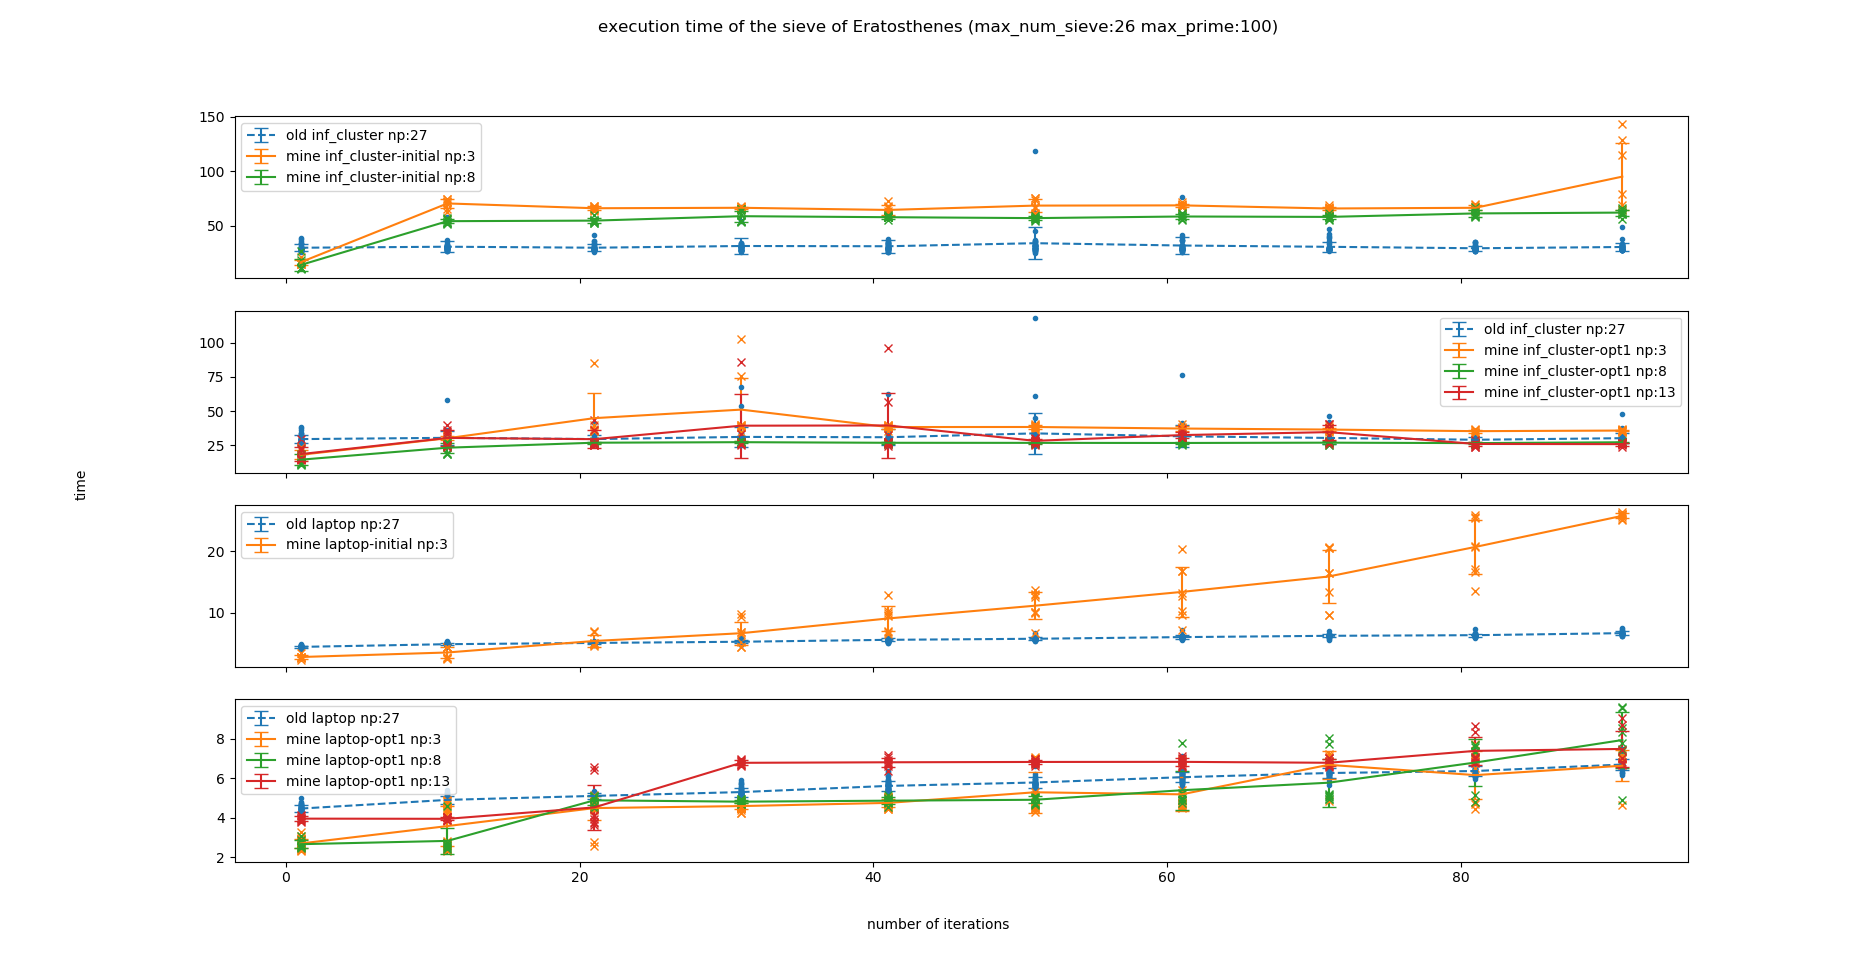
\includegraphics[width=1\textwidth]{figures/sieve_all_100}
    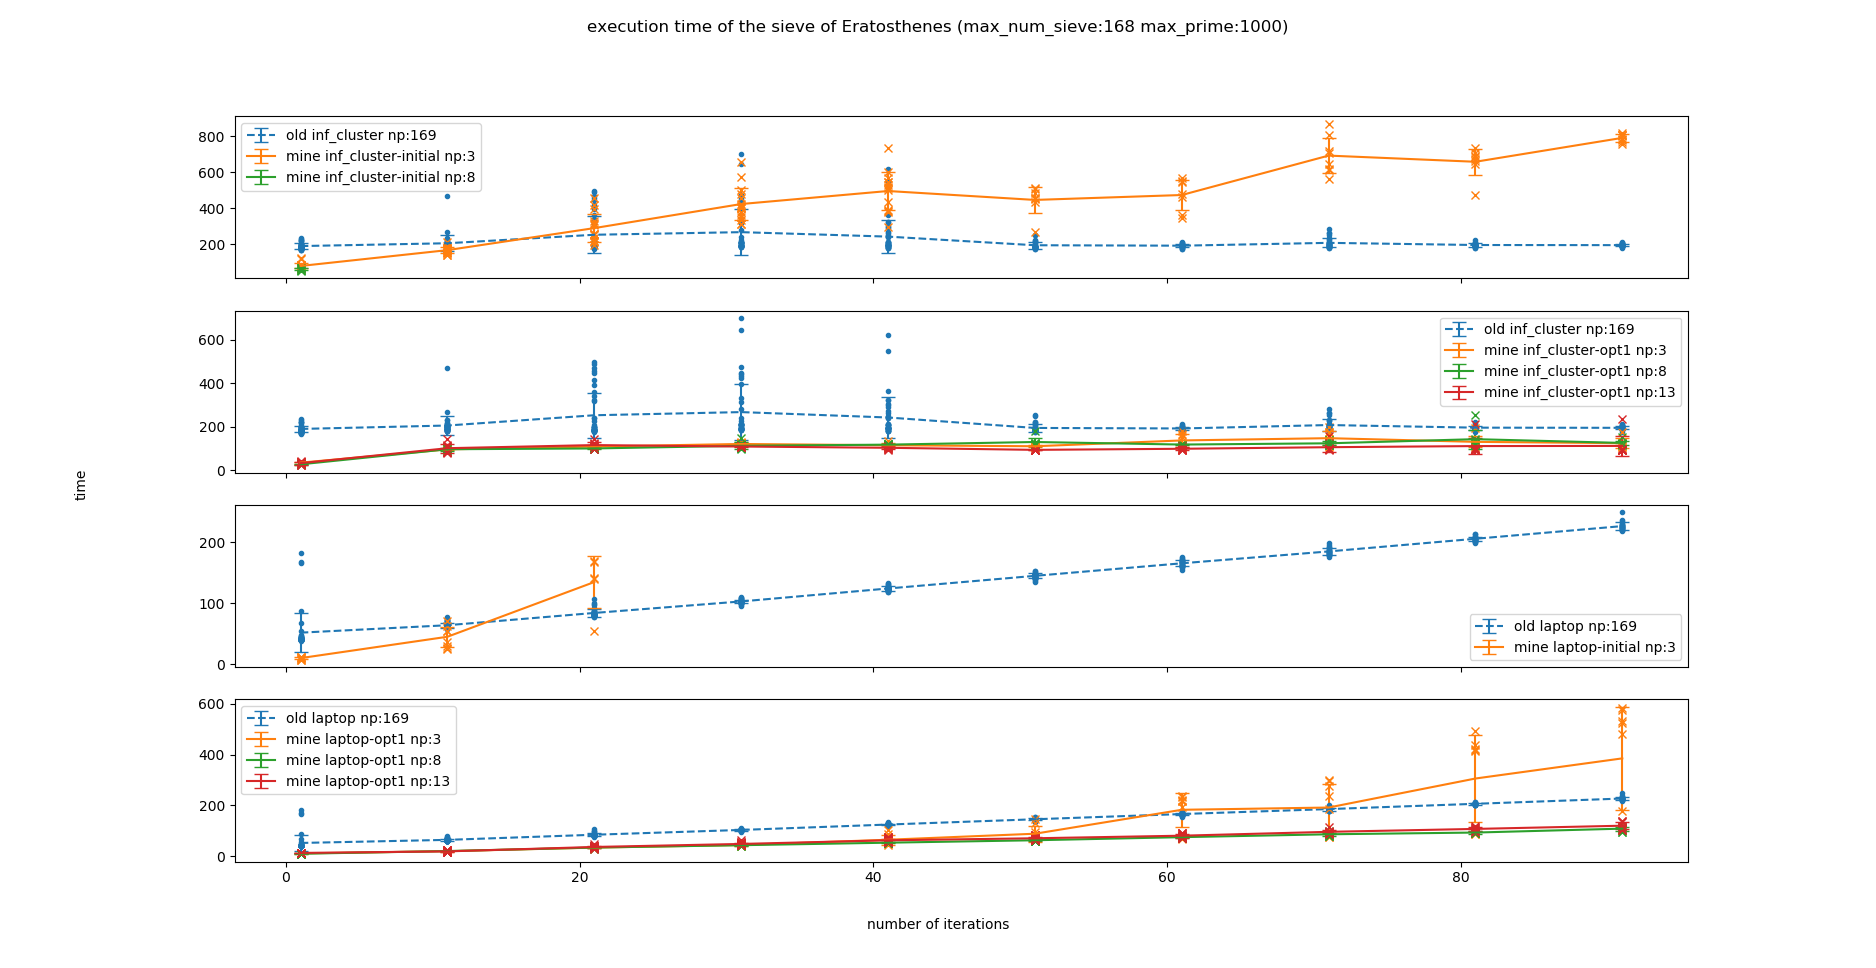
\includegraphics[width=1\textwidth]{figures/sieve_all_1000}
	\caption{Execution time of the sieve of Eratothesnes on both the old semantics and our new semantics.
	The second column of the legend indicates the platform and the version (separated by a dash), and the third column of the legend is one of the parameters controlling the number of nodes spawned at the beginning}
	\label{fig:sieve_all}
\end{figure}

\begin{figure}[h]
	\centering
    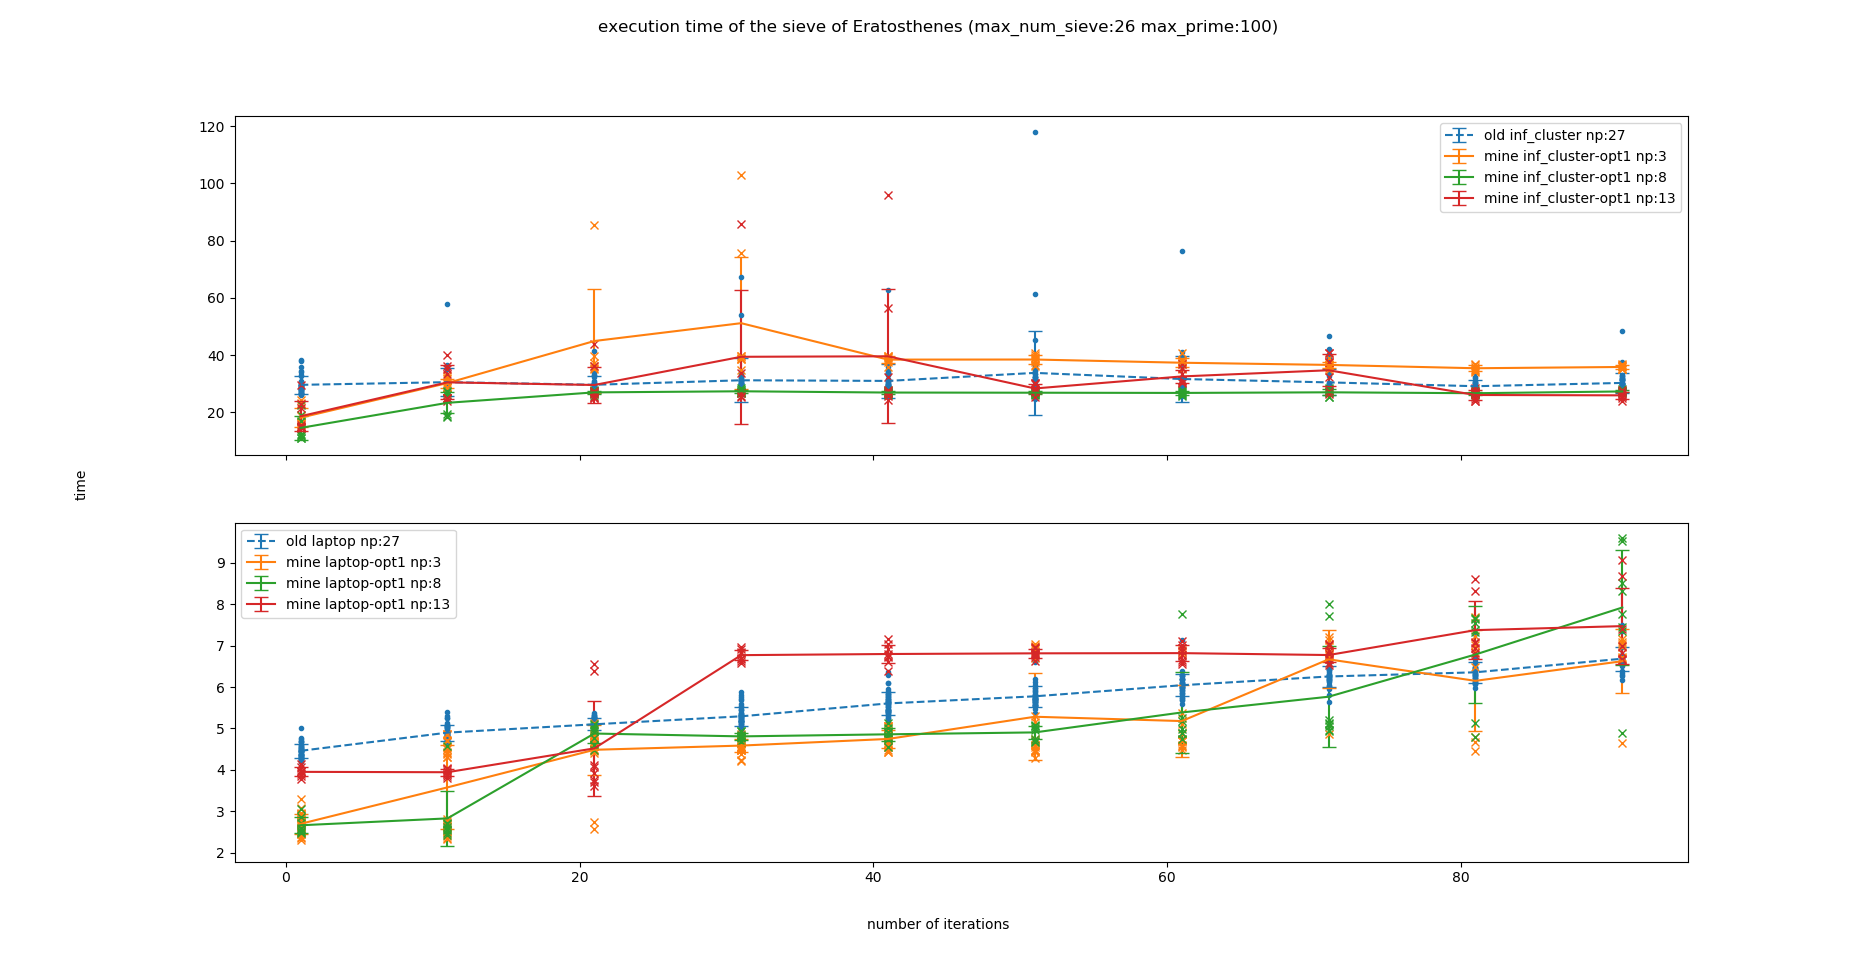
\includegraphics[width=1\textwidth]{figures/sieve_opt1_100}
    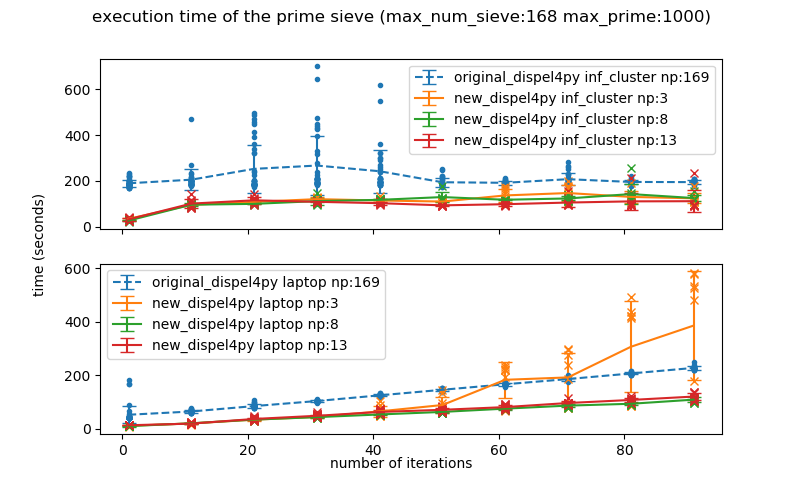
\includegraphics[width=1\textwidth]{figures/sieve_opt1_1000}
	\caption{Execution time of the sieve of Eratothesnes on both the old semantics and our new semantics (only the optimized version)}
	\label{fig:sieve_opt1}
\end{figure}
	
	\section{Conclusion}
	\sout{What we have done. How good or bad are them. What further work can be done.}
	
	
	\pagebreak
	\bibliography{dissertation_bib}
	\bibliographystyle{plain}
\end{document}